%*******************************************************************************
% Example chapter file for books, Copyright A K Peters, Ltd.
%*******************************************************************************
\chapter{Depth of Field with Bokeh Rendering}{Charles de Rousiers and Matt Pettineo}
\label{BokehRendering}

%-------------------------------------------------------------------------------
\section{Introduction}

In order to increase realism and immersion, current games make frequent use of depth of field to simulate lenticular phenomena. Typical implementations use screen-space filtering techniques to roughly approximate a camera's circle of confusion for out-of-focus portions of a scene. While such approaches can provide pleasing results with minimal performance impact, crucial features present in real-life photography are still missing. In particular, lens-based cameras produce a phenomenon known as \bokeh\index{bokeh} (blur in Japanese). Bokeh manifests as distinctive geometric shapes that are most visible in out-of-focus portions of an image with high local contrast. The actual shape itself depends on the shape of the camera’s aperture, which is typically circular, octagonal, hexagonal, or pentagonal.

	\begin{figure}[htb]\centering
	\includegraphics[width=\textwidth]{montage2.png}
	\caption{Comparison between a simple blur-based depth of field (left) and a depth of field with bokeh rendering (right). }
	\label{Derousiers:blurcomparison}
	\end{figure}

Current and upcoming DirectX 11 engines, i.e. CryENGINE, Unreal Engine 3, etc, have recently demonstrated new techniques for simulating bokeh depth of field, which reflects a rising interest in reproducing such effects in real-time. However, these techniques have performance requirements that can potentially relegate them to high-end GPU's. The precise implementation details of these techniques also aren't publicly available, making it difficult to integrate these techniques into existing engines. Consequently it remains an active area of research, as there is still a need for implementations that are suitable for a wider range of hardware.

A naive approach would be to explicitly render a quad for each pixel, with each quad using a texture containing the aperture shape. While this can produce excellent results, it's also extremely inefficient due to the heavy fillrate and bandwidth requirements. Instead, we propose a hybrid method which mixes previous filtering-based approaches with quad rendering. Our method selects pixels with high local contrast, and renders a single textured quad for each such pixel. The texture used for the quad contains the camera's aperture shape, which allows the quads to approximate bokeh effects. In order to achieve high performance, we use atomic counters in conjunction with an image texture for random memory access. An indirect draw command is also used, which avoids the need for expensive CPU / GPU synchronization. This efficient OpenGL 4.2 implementation allows rendering of thousands of aperture-shaped quads at high frame-rates, and also ensures the temporal coherency of the rendered \bokeh.

%-------------------------------------------------------------------------------
\section{Depth of Field Phenomemon}\label{Derousiers:DOFPhenomenon}
Depth of field\index{depth of field} is an important effect for conveying a realistic sense of depth and scale, particularly in open scenes with a large viewing distance. Traditional real-time applications use a pinhole camera model for rasterization, which results in an infinite depth of field. However real cameras use a thin lens, which introduces a limited depth of field based on aperture size and focal distance. Objects outside of this of this region appear blurred on the final image, while objects inside of it remain sharp. See Figure~\ref{Derousiers:focus}.

	\begin{figure}[htb]\centering
	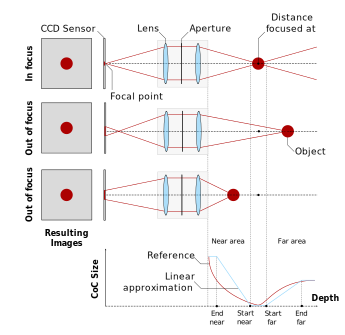
\includegraphics[width=\textwidth]{focus}
	\caption{Depth of field phenomenon, where a thin lens introduces a limited depth of field. In-focus objects appear sharp, while out-of-focus object appear blurred. The size of the circle of confusion depends on the distance beween object and the point at which the camera is focused. We use a linear approximation in order to simplify parameters and as well as run-time computations. }
	\label{Derousiers:focus}
	\end{figure}


The ``blurriness" of an object is defined by its \emph{circle of confusion} (\coc). The size of this \coc depends on the distance between the object and the area at which the camera is focused. The further an object is from the focused area, the blurrier it appears. The size of the \coc does not increase linearly based on this distance. The size actually increases faster in the out-of-focus foreground area than it does the out-of-focus background area, see Figure~\ref{Derousiers:focus}. Since the \coc size ultimately depends on focal distance, lens size, and aperture shape, setting up the simulation parameters may not be intuitive to someone inexperienced with photography. This is why we use a simple linear approximation as proposed by~\cite{Hammon07}, see Figure~\ref{Derousiers:focus}.

	\begin{figure}[htb]\centering
	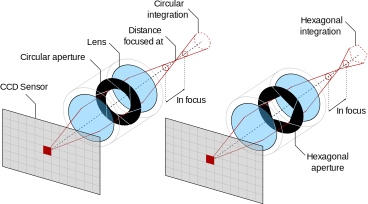
\includegraphics[width=\textwidth]{camera}
	\caption{Aperture shape of a camera. Aperture blocks a portion of the incoming light. Its shape modifies the pixel integration, and hence, it changes the \bokeh shape. }
	\label{Derousiers:camera}
	\end{figure}

The \textit{aperture}\index{aperture} of a camera is responsible for allowing light to pass through the lens and strike the sensor (or film)\footnote{If an object or the camera moves while the aperture is open, the objects will appear blurred. This is known as motion blur.}. The shape of this aperture directly impacts the formation of the image, since each out-of-focus point is convolved with the aperture shape. See Figure~\ref{Derousiers:camera}.

While it is often difficult to see distinct \bokeh patterns in areas with low contrast, \bokeh is clearly visible in areas that are significantly brighter than their surroundings. We use this observation as a heuristic to determine where \bokeh quads need to be drawn in order to provide a plausible approximation.

%-------------------------------------------------------------------------------
\section{Related Work}\label{Derousiers:RelativeWork}

Several methods have been proposed during the last decade for efficiently approximating a depth of field effect. However those methods use a Gaussian blur or heat diffusion to simulate out-of-focus areas~\cite{Hammon07,Kosloff07} and are therefore unable to reproduce \bokeh effects.

An earlier approach from Krivanek~\cite{Krivanek03} uses sprite splatting as a means for implementing depth of field, rather than a filtering approach. While this brute force method does produce \bokeh shapes, it is quite inefficient due to excessive overdraw and bandwidth consumption. The video games industry has shown a recent interest for \bokeh effects~\cite{Sousa11,Futurmark11,Mittring11}. While complete implementation details are not available, these methods largely take a similar approach as Krivanek where sprites are rendered for each pixel. Consequently, these techniques make use of complex optimizations, i.e. hierarchical rasterization, multiple downscaling passes, etc, in order to improve performance. 

A recent approach proposed by White~\cite{White11} reproduces hexagonal \bokeh using several directional blur passes. While efficient, this method does not support arbitrary aperture shapes.

%-------------------------------------------------------------------------------
\section{Algorithm}
We observe that only points with a high local contrast will produce distinct \bokeh shapes. We use this heuristic to detect \bokeh positions in screen space~\cite{Pettineo11} and then splat textured quads at those locations. The remaining pixels use a blur-based approach to simulate a circle of confusion.

\subsection{Overview}
Our approach is divided into four passes, see Figure~\ref{Derousiers:pipeline}. The first pass computes the \coc size for each pixel based on its depth value, and then outputs a linear depth value to a render target texture\footnote{If a linear depth buffer is available as an input, the first two passes can be merged together.}. Then, the second pass computes the contrast of the current pixel by comparing the pixel's brightness with the brightness of the 5x5 neighboring pixels. If this contrast is above a pre-defined threshold, its position, \coc size, and average color are appended to a buffer. During the third pass, a blur-based depth of field is computed with one of the previous methods, i.e. Gaussian blur, etc. Finally, a fourth pass splats textured quads at the \bokeh positions that were appended to the buffer in the second pass.

	\begin{figure}[htb]\centering
	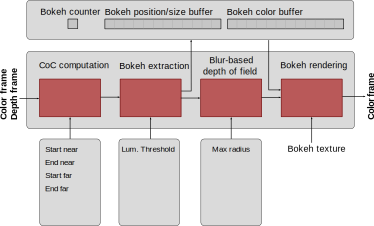
\includegraphics[width=\textwidth]{pipeline}
	\caption{Overview of the pipeline. It is composed of four passes, and takes as input the color and depth buffers of the current frame. It outputs a final color image with depth of field and \bokeh effects.}
	\label{Derousiers:pipeline}
	\end{figure}

In order to maintain high performance, it is crucial to avoid CPU/GPU synchronization. We ensure this by making use of an indirect draw command, which renders a number of quads based on the count stored in the append buffer. This way, the number of \bokeh points detected by the CPU is never read back by the CPU.

\subsection{Circle of confusion computation}
Setting up depth of field using physical camera parameters, such as focal length and aperture size, can be non-intuitive for those not familiar with optics or photography. Instead, we define two areas where geometry is out-of-focus: a near/foreground area and a far/background area. Both areas are delimited with a near and far depth values, see Figure~\ref{Derousiers:focus}. In both regions, the blur amount is linearly interpolated between the two bounds. This allows a simple and intuitive means of describing the depth of field for a given scene.

$$
	CoC = \frac{Z_{pixel} - Z_{start} }{ Z_{end} - Z_{start} }
$$

The resulting \coc size from this equation is normalized to [0,1]. An extra parameter \codecmd{MaxRadius} determines a posteriori what the final size of the blur will be in screen space. This setting can be tweaked by artists in order to achieve the desired appearance, and provides a mean of balancing performance: smaller values of \codecmd{MaxRadius} result in greater performance.


\subsection{\Bokeh detection}
The detection pass aims to detect pixels from which we will generate \bokeh shapes. To detect such pixels, we use the following heuristic : \emph{a pixel with high contrast in a given neighborhood will generate a \bokeh shape}. We compare the current pixel luminance $L_{pixel}$ to its neighborhood luminance $L_{neigh}$. If the difference $L_{pixel}-L_{neigh}$ is greater than the threshold \codecmd{LumThreshold}, then the current pixel is registered as a \bokeh point\footnote{We also use the threshold \codecmd{CoCThreshold to discard bokeh with a small radius.}}. Pixels detected as \bokeh are sparse, which means writing them into a render target texture would be wasteful in terms of both memory usage and bandwidth. To address this problem, we use the \opengl \codecmd{ImageBuffers}\index{image buffer} in combination with an \codecmd{AtomicCounter}\index{atomic counter}. This allows us to build a vector in which we append parameters for detected \bokeh points. \codecmd{ImageBuffers} have to be preallocated with a given size, i.e. the maximum number of \bokeh sprites that can be displayed on screen. The atomic counter \codecmd{BokehCounter} stores the number of appended \bokeh points. Its current value indicates the next free cell in the \codecmd{ImageBuffers} vector. Two \codecmd{ImageBuffers}, \codecmd{BokehPosition} and \codecmd{BokehColor}, are used to store \coc size, position, and color of the detected \bokeh points. See Listings \ref{Derousiers:bokehextractioncpp} and \ref{Derousiers:bokehextractionfs}.

	\begin{figure}[htb]\centering
	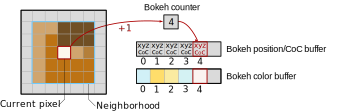
\includegraphics[width=0.8\textwidth]{extraction}
	\caption{\Bokeh detection. The luminance of the current pixel is compared to its neighborhood. If the difference is greater than \codecmd{LunThreshod}, \bokeh parameters, i.e position, color, and \coc, are appended into \codecmd{BokehPosition} and \codecmd{BokehColor} buffers. The atomic counter \codecmd{BokehCounter} is also incremented.}
	\label{Derousiers:detection}
	\end{figure}

\subsection{Blur-based depth of field}
Several approaches are possible for this pass. We refer readers to previous work for this step. Nevertheless, here is a short summary of popular approaches:
\begin{itemize}
	\item Perform a Gaussian blur with fixed kernel width at various resolutions, and apply a linear interpolation to blend them according to \coc size.
	\item Perform a Poisson disc sampling in screen space, with radius determined by pixel \coc size~\footnote{A random rotation can be applied to a Poisson sampling pattern for transforming aliasing into noise.}.
	\item Apply a large-width bilateral filter where invalid pixels are rejected based on depth~\footnote{For implementation details, we refer the reader to the code sample. This approach offers a good compromise between quality and performances. However, larger filter kernels require a large sampling radius. An \opencl implementation would allow for better performance, since shared memory can be used to cache texture fetches.}.
\end{itemize}


\subsection{\Bokeh rendering}
In order to avoid CPU/GPU synchronization, we use the indirect drawing command \codecmd{glDrawArraysIndirect}. This command draws instances of a given VBO/VAO, where the number of instances is read from a buffer located in GPU memory. This buffer can be updated from either the CPU or the GPU. In order to allow the GPU to operate independently of the CPU, we update this buffer from the GPU before the last pass. We bind this indirect buffer as a \codecmd{ImageTexture} and copy the value of the atomic counter into it. Thus, the number of instances drawn is equal to the number of detected \bokeh points, see Listings \ref{Derousiers:synchronizationbokehfs} and \ref{Derousiers:renderingbokehcpp}.

We use this command in combination with a point VAO. The instanced points are translated by the vertex shader such that they are located at the screen space \bokeh position. This position is read from the \codecmd{BokehPosition} buffer, which is indexed using the built-in \codecmd{gl\_InstanceID} input variable. After being transformed in the vertex shader, each point is expanded into a quad in the geometry shader. The size of this quad is determined by the \bokeh size which is also read from the \codecmd{BokehPosition} buffer. Finally, the fragment shader applies the \bokeh alpha-texture onto the quad and multiplies it by the \bokeh color which is read from the \codecmd{BokehColor} buffer. See Listings \ref{Derousiers:renderingbokehvs}, \ref{Derousiers:renderingbokehgs}, and \ref{Derousiers:renderingbokehfs}.

%-------------------------------------------------------------------------------
\section{Results}
Figures \ref{Derousiers:blurcomparison}, \ref{Derousiers:bokehrendering}, and \ref{Derousiers:bokehcomparison} show the rendering of a tank with our method. Since the final bokeh shape is texture-driven, we can apply arbitrary shapes. See Figure \ref{Derousiers:bokehcomparison}.

	\begin{figure}[htb]\centering
	\includegraphics[width=\textwidth]{screen3.png}
	\caption{Rendering of a tank with a small depth of field. Bokeh shapes are clearly visible on the more reflective surfaces of the tank.}
	\label{Derousiers:bokehrendering}
	\end{figure}

	\begin{figure}[htb]\centering
	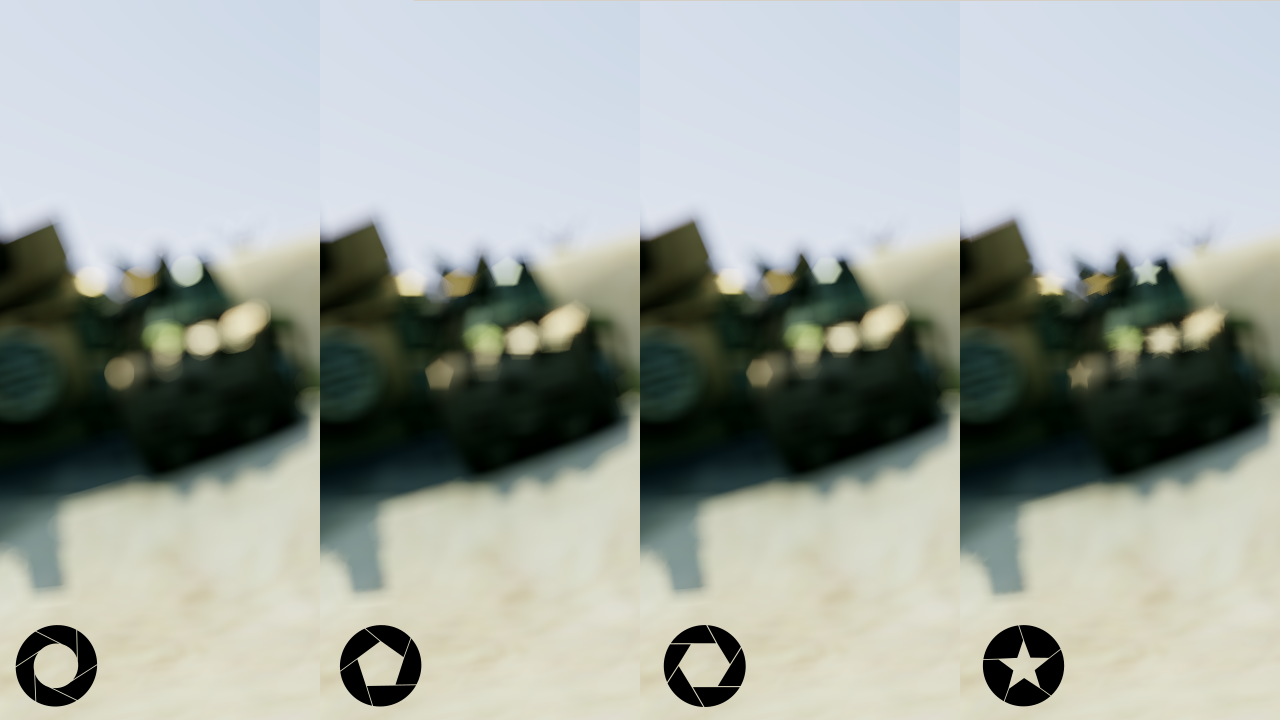
\includegraphics[width=\textwidth]{montage.pdf}
	\caption{Rendering of the same scene with different aperture shapes. From left to right: a circle aperture, a pentagonal aperture, an hexagonal aperture, and a star aperture.}
	\label{Derousiers:bokehcomparison}
	\end{figure}

Figure \ref{Derousiers:performance} details the rendering times of each pass as well as the the number of detected \bokeh points. We can see that the blur-based depth of field pass is the most expensive, indicating that a more optimal approach might be more suitable. Unlike the blur and detection passes, the rendering pass is strongly dependent on the number of detected \bokeh points. Under normal conditions, our algorithm detects around 5,000 \bokeh points in the the tank scene. In the case, the cost of the rendering pass is less than 2 milliseconds.

	\begin{figure}[htb]\centering
	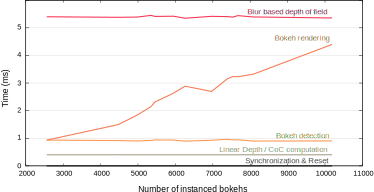
\includegraphics[width=\textwidth]{performances}
	\caption{Timings of the different passes for varying numbers of detected \bokeh points. Those timings have been recorded on a nVidia GeForce 580GTX at 1280x720. }
	\label{Derousiers:performance}
	\end{figure}

%-------------------------------------------------------------------------------
\section{Discussion}
Temporal coherence is a natural concern for this approach. Like other methods, we base our approach on the final color buffer. If sub-pixel aliasing is addressed by previous rendering steps, our approach is stable, and \bokeh shapes are coherent from frame-to-frame. In the case of sub-pixel aliasing, our method exhibits the same limitations as all previous methods, and the resulting \bokeh shapes may flicker.

Also, our method requires preallocated buffers for storing the \bokeh position and color. Consequently, a maximum number of \bokeh points has to be specified. If this number is too low, \bokeh points may pop and flicker from frame-to-frame with little coherency. If this number is too large, then GPU memory is potentially wasted. Thus, the maximum number of sprites must be carefully chosen to suit the type of scene being displayed.

%-------------------------------------------------------------------------------
\section{Conclusion}
We have presented an efficient implementation for rendering a depth of field effect with \bokeh. This method allows us to combine an efficient blur-based approach with plausible \bokeh reproduction. We use a heuristic to identify pixels that produce distinct \bokeh shapes, and then render those shapes as textured quads. This implementation avoids costly CPU/GPU synchronization through the use of indirect draw commands. These commands allow the GPU to directly read the number of instances, without the need for CPU readback.

While this approach provides good visual results, several optimizations can be made in order to improve performance. In particular, large \coc sizes requires rasterization of quads that cover a significant portion of the screen. Using hierarchical rasterization, as proposed in~\cite{Futurmark11}, could improve performance by reducing the number of pixels that need to be shaded and blended.



\begin{lstlisting}[language=C++,float={htb},caption={Host application for extracting \bokehs \emph{(Pass 2)}.},label={Derousiers:bokehextractioncpp}]
		// Indirect buffer definition
		struct DrawArraysIndirectCommand
		{
			GLuint count;
			GLuint primCount;
			GLuint first;
			GLuint reservedMustBeZero;
		};

		// Create indirect buffer
		GLuint indirectBufferID;
		glGenBuffers(1,&indirectBufferID);
		glBindBuffer(GL_DRAW_INDIRECT_BUFFER,indirectBufferID);
		DrawArraysIndirectCommand indirectCmd;
		indirectCmd.count              = 1;
		indirectCmd.primCount          = 0;
		indirectCmd.first              = 0;
		indirectCmd.reservedMustBeZero = 0;
		glBufferData(GL_DRAW_INDIRECT_BUFFER,sizeof(DrawArraysIndirectCommand),&indirecCmd,GL_DYNAMIC_DRAW);

		// Create a texture proxy for the indirect buffer 
		// (for using it as an atomic counter)
		glGenTextures(1, &bokehCountTexID);
		glBindTexture(GL_TEXTURE_BUFFER, bokehCountTexID);
		glTexBuffer(GL_TEXTURE_BUFFER, GL_R32UI, pointIndirectBuffer.id);

		// Create atomic counter
		glGenBuffers(1,&bokehCounter);
		glBindBuffer(GL_ATOMIC_COUNTER_BUFFER,bokehCounter);
		glBufferData(GL_ATOMIC_COUNTER_BUFFER,sizeof(unsigned int),0,GL_DYNAMIC_DRAW);

		// Create position and color textures with a GL_RGBA32F inner format
		...

		// Bind atomic counter
		glBindBufferBase(GL_ATOMIC_COUNTER_BUFFER,0,bokehCounter);

		// Bind position image buffer
		glActiveTexture(GL_TEXTURE0 + bokehPosionTexUnit);
		glBindImageTexture(bokehPostionTexUnit,bokehPositionTex.id,0,false,0,GL_WRITE_ONLY,GL_RGBA32F);

		// Bind color image buffer
		glActiveTexture(GL_TEXTURE0 + bokehColorTexUnit);
		glBindImageTexture(bokehColorTexUnit,bokehColorTex.id,0,false,0,GL_WRITE_ONLY,GL_RGBA32F);

		DrawSceenQuad();
\end{lstlisting}


\begin{lstlisting}[language=GLSL,float={htb},caption={Fragment shader for extracting \bokehs \emph{(Pass 2)}.},label={Derousiers:bokehextractionfs}]	
	#version 420
	// Bokeh counter, position (x,y,z,size), and color
	layout(binding=0,offset=0) uniform atomic_uint BokehCounter;
	layout(size4x32) writeonly uniform image1D BokehPositionTex;
	layout(size4x32) writeonly uniform image1D BokehColorTex;

	// Constrast and CoC thresholds
	uniform float LumThreshold;
	uniform float CoCThreshold;
	...

	float  cocCenter; // Current CoC size
	vec3 colorCenter; // Current pixel color
	vec3 colorNeighs; // Average color of the neighborhood

	// Append pixel whose constrast is greater than the user's threshold
	float lumNeighs = dot(colorNeighs, vec3(0.299f, 0.587f, 0.114f));
	float lumCenter = dot(colorCenter, vec3(0.299f, 0.587f, 0.114f));
	if((lumCenter-lumNeighs)>LumThreshold && cocCenter>CoCThreshold)
	{
		int current = int(atomicCounterIncrement(BokehCounter));
		imageStore(BokehPositionTex,current,vec4(gl_FragCoord.x,gl_FragCoord.y,depth,cocCenter));
		imageStore(BokehColorTex,current,vec4(colorCenter,1));
	}
\end{lstlisting}

\begin{lstlisting}[language=GLSL,float={htb},caption={Synchronization of the indirect buffer with the atomic counter \emph{(Pass 3/4)}.},label={Derousiers:synchronizationbokehfs}]
	#version 420
	layout(binding=0,offset=0) uniform atomic_uint BokehCounter;
	layout(size1x32) writeonly uniform uimage1D IndirectBufferTex;
	out vec4 FragColor;

	void main()
	{
	imageStore(IndirectBufferTex,1,uvec4(atomicCounter(BokehCounter),0,0,0));
	FragColor = vec4(0);
	}
\end{lstlisting}

\begin{lstlisting}[language=C++,float={htb},caption={Host application for rendering bokeh \emph{(Pass 4)}.},label={Derousiers:renderingbokehcpp}]
	// Create point VBO
	GLuint pointVboID;
	glm::vec3 defaultPosition(0,0,0);
	glGenBuffers(1,&pointVboID);
	glBindBuffer(GL_ARRAY_BUFFER,pointVboID);
	glBufferData(GL_ARRAY_BUFFER,sizeof(glm::vec3),&defaultPosition,GL_STATIC_DRAW);

	// Create point VAO
	GLuint pointVaoID;
	glGenVertexArrays(1, &pointVaoID);
	glBindVertexArray(pointVaoID);
	glVertexAttribPointer(semantic::PositionLocation,3, GL_RGB,false,GL_FLOAT,GLF_BUFFER_OFFSET(_offset));
	glEnableVertexAttribArray(semantic::PositionLocation);
	glBindBuffer(GL_ARRAY_BUFFER, 0);
	glBindVertexArray(0);
	...

	// Wait for atomic counter synchronization and draw bokehs
	glMemoryBarrier(GL_ALL_BARRIER_BITS);
	glUseProgram(bokehRenderingProgramID);

	glActiveTexture(GL_TEXTURE0 + bokehShapeTexUnit);
	glBindTexture(GL_TEXTURE_1D,bokehShapeTexID);
	glActiveTexture(GL_TEXTURE0 + bokehColorTexUnit);

	glBindTexture(GL_TEXTURE_1D,bokehColorTexID);
	glActiveTexture(GL_TEXTURE0 + bokehPositionTexUnit);
	glBindTexture(GL_TEXTURE_1D,bokehPositionTexID);

	glBindVertexArray(pointVaoID);
		glBindBuffer(GL_DRAW_INDIRECT_BUFFER,indirectBufferID);
		glDrawArraysIndirect(GL_POINTS,NULL);
		glBindBuffer(GL_DRAW_INDIRECT_BUFFER,0);
	glBindVertexArray(0);
\end{lstlisting}


\begin{lstlisting}[language=C++,float={htb},caption={Pixel shader application for rendering bokeh \emph{(Pass 4)}.},label={Derousiers:renderingbokehvs}]
#version 420
uniform vec2      PixelScale;       // (1/xResolution,1/yResolution)
uniform sampler1D BokehPositionTex; // (x,y,z,scale)
uniform sampler1D BokehColorTex;
in vec3           Position;
out float         vRadius;
out vec4          vColor;

int main()
{
	vec3 pos     = texelFetch(BokehPositionTex,gl_InstanceID,0).xyzw;
	vRadius      = pos.w;
	vColor       = texelFetch(BokehColorTex,gl_InstanceID,0);
	gl_Position	 = vec4((Position.xy+pos.xy)*PixelScale,0,1);
}
\end{lstlisting}

\begin{lstlisting}[language=GLSL,float={htb},caption={Geometry shader for rendering bokeh \emph{(Pass 4)}.},label={Derousiers:renderingbokehgs}]
#version 420
uniform mat4     Transformation;
uniform vec2     PixelScale;
in  float        vRadius[1];
in  vec4         vColor[1];
out vec4         gColor;
out vec2         gTexCoord;
layout(points)   in;
layout(triangle_strip, max_vertices = 6) out;

void main()
{
	gl_Layer     = 0;
	vec4 offsetx = vec4(PixelScale.x*Radius[0],0,0,0);
	vec4 offsety = vec4(0,PixelScale.y*Radius[0],0,0);
	gColor       = vColor[0];
	gl_Position  = Transformation*(gl_in[0].gl_Position-offsetx-offsety);
	gTexCoord    = vec2(0,0);
	EmitVertex();
	gl_Position  = Transformation*(gl_in[0].gl_Position+offsetx-offsety);
	gTexCoord    = vec2(1,0);
	EmitVertex();
	gl_Position  = Transformation*(gl_in[0].gl_Position-offsetx+offsety);
	gTexCoord    = vec2(0,1);
	EmitVertex();
	gl_Position  = Transformation*(gl_in[0].gl_Position+offsetx+offsety);
	gTexCoord    = vec2(1,1);
	EmitVertex();
	EndPrimitive();
}
\end{lstlisting}

\begin{lstlisting}[language=GLSL,float={htb},caption={Fragment shader for rendering bokeh \emph{(Pass 4)}.},label={Derousiers:renderingbokehfs}]
#version 420
uniform sampler2D    BokehShapeTex; // Bokeh shape texture
in  vec4             gColor;
in  vec2             gTexCoord;
out vec4             FragColor;
void main()
{
	FragColor = vec4(gColor.xyz*texture(BokehShapeTex,gTexCoord).x,gColor.w);
}
\end{lstlisting}



%-------------------------------------------------------------------------------
\bibliographystyle{akpbib}
\bibliography{BokehRendering}











